\begin{figure*}[tp]
\centering
\begin{tikzpicture}
\begin{axis}[
    width=0.8\textwidth,
    height=0.4\textwidth,
    xlabel=Search Depth,
    ylabel=Cumulative Value,
    grid=major,
    clip=false,
    xmode=log,
    log basis x=2,
    xtick={1,2,4,8,16,32,64},
    xticklabels={$2^0$,$2^1$,$2^2$,$2^3$,$2^4$,$2^5$,$2^6$},
    xmin=1,
]
\addplot[name path=upper, draw=none] coordinates {
(0,505.5464607176052)
(1,1130.7662111899358)
(2,1402.4081585979516)
(3,1951.6058732475399)
(4,2346.3712658611407)
(5,2485.755370868389)
(6,2553.8514321848356)
(7,2659.896180048888)
(8,2935.5680415257807)
(9,3067.8206628136572)
(10,3408.79612497651)
(11,3763.9023615181045)
(12,4062.0889663718126)
(13,4191.518914692166)
(14,4201.081167647662)
(15,4147.61803398875)
(16,4272.95778063328)
(17,4585.077924342993)
(18,4821.08054277059)
(19,5141.560141085828)
(20,5402.468011357288)
(21,6028.9886756603)
(22,6731.636071520627)
(23,7115.735545569184)
(24,7389.234982301745)
(25,7782.393473354603)
(26,7988.537869130834)
(27,8178.257701234411)
(28,8662.51952529317)
(29,8838.628082789173)
(30,9074.101504081475)
(31,9342.013946828205)
};
\addplot[name path=lower, draw=none] coordinates {
(0,405.9535392823948)
(1,1011.2337888100643)
(2,1235.0918414020484)
(3,1689.3941267524601)
(4,2091.1287341388593)
(5,2357.744629131611)
(6,2534.6485678151644)
(7,2631.103819951112)
(8,2902.4319584742193)
(9,3026.1793371863428)
(10,3301.70387502349)
(11,3641.0976384818955)
(12,3841.4110336281874)
(13,3946.9810853078347)
(14,4120.918832352338)
(15,4145.38196601125)
(16,4119.04221936672)
(17,4398.922075657007)
(18,4639.41945722941)
(19,4954.439858914172)
(20,5316.531988642712)
(21,5598.5113243397)
(22,6123.363928479373)
(23,6955.764454430816)
(24,7235.265017698255)
(25,7685.106526645397)
(26,7839.962130869166)
(27,7861.742298765589)
(28,8598.48047470683)
(29,8782.871917210827)
(30,8964.398495918525)
(31,9225.486053171795)
};
\addplot[blue!20, opacity=0.3] fill between[of=upper and lower];
\addplot[blue, thick] coordinates {
(0,455.75)
(1,1071.0)
(2,1318.75)
(3,1820.5)
(4,2218.75)
(5,2421.75)
(6,2544.25)
(7,2645.5)
(8,2919.0)
(9,3047.0)
(10,3355.25)
(11,3702.5)
(12,3951.75)
(13,4069.25)
(14,4161.0)
(15,4146.5)
(16,4196.0)
(17,4492.0)
(18,4730.25)
(19,5048.0)
(20,5359.5)
(21,5813.75)
(22,6427.5)
(23,7035.75)
(24,7312.25)
(25,7733.75)
(26,7914.25)
(27,8020.0)
(28,8630.5)
(29,8810.75)
(30,9019.25)
(31,9283.75)
};
\node at (axis cs:1,-956.73) {
    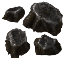
\includegraphics[width=1em]{icons/coal.png}
};
\node at (axis cs:1,-250.49) {
    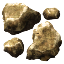
\includegraphics[width=1em]{icons/stone.png}
};
\node at (axis cs:1,455.75) {
    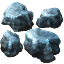
\includegraphics[width=1em]{icons/iron-ore.png}
};
\node at (axis cs:1,1161.9900000000002) {
    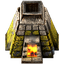
\includegraphics[width=1em]{icons/stone-furnace.png}
};
\node at (axis cs:1,1868.23) {
    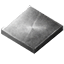
\includegraphics[width=1em]{icons/iron-plate.png}
};
\node at (axis cs:2,1318.75) {
    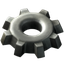
\includegraphics[width=1em]{icons/iron-gear-wheel.png}
};
\node at (axis cs:7,2292.38) {
    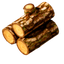
\includegraphics[width=1em]{icons/wood.png}
};
\node at (axis cs:7,2998.62) {
    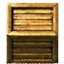
\includegraphics[width=1em]{icons/wooden-chest.png}
};
\node at (axis cs:9,3047.0) {
    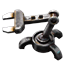
\includegraphics[width=1em]{icons/burner-inserter.png}
};
\node at (axis cs:12,3951.75) {
    
\includegraphics[width=1em]{icons/transport-belt.png}
};
\node at (axis cs:21,5813.75) {
    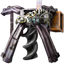
\includegraphics[width=1em]{icons/burner-mining-drill.png}
};
\end{axis}
\end{tikzpicture}
\caption{MCTS progression showing cumulative value and item achievements}
\label{fig:mcts-progression}
\end{figure*}